\chapter{Configuración de impresora}\label{chap:apendiceA}
Para comenzar con el trabajo de impresión, se debió leer y entender el manual de procedimientos incluido con el dispositivo \cite{DimatixUM}. A su vez, dada la alta complejidad de estos trabajos se analizaron publicaciones realizadas en la Universidad de Pennsylvania \cite{UPenn} y en la Universidad de Michigan \cite{UMic}, donde se explica con mayor detalle las calibraciones y manejo de muestras.

La impresora (Figura ~\ref{fig:Figura_Impresora_DMP2850}) consta de una platina con sistema de vacío para sujeción de muestras y un sistema calefactor. 

\begin{figure}[H]
  \centering
    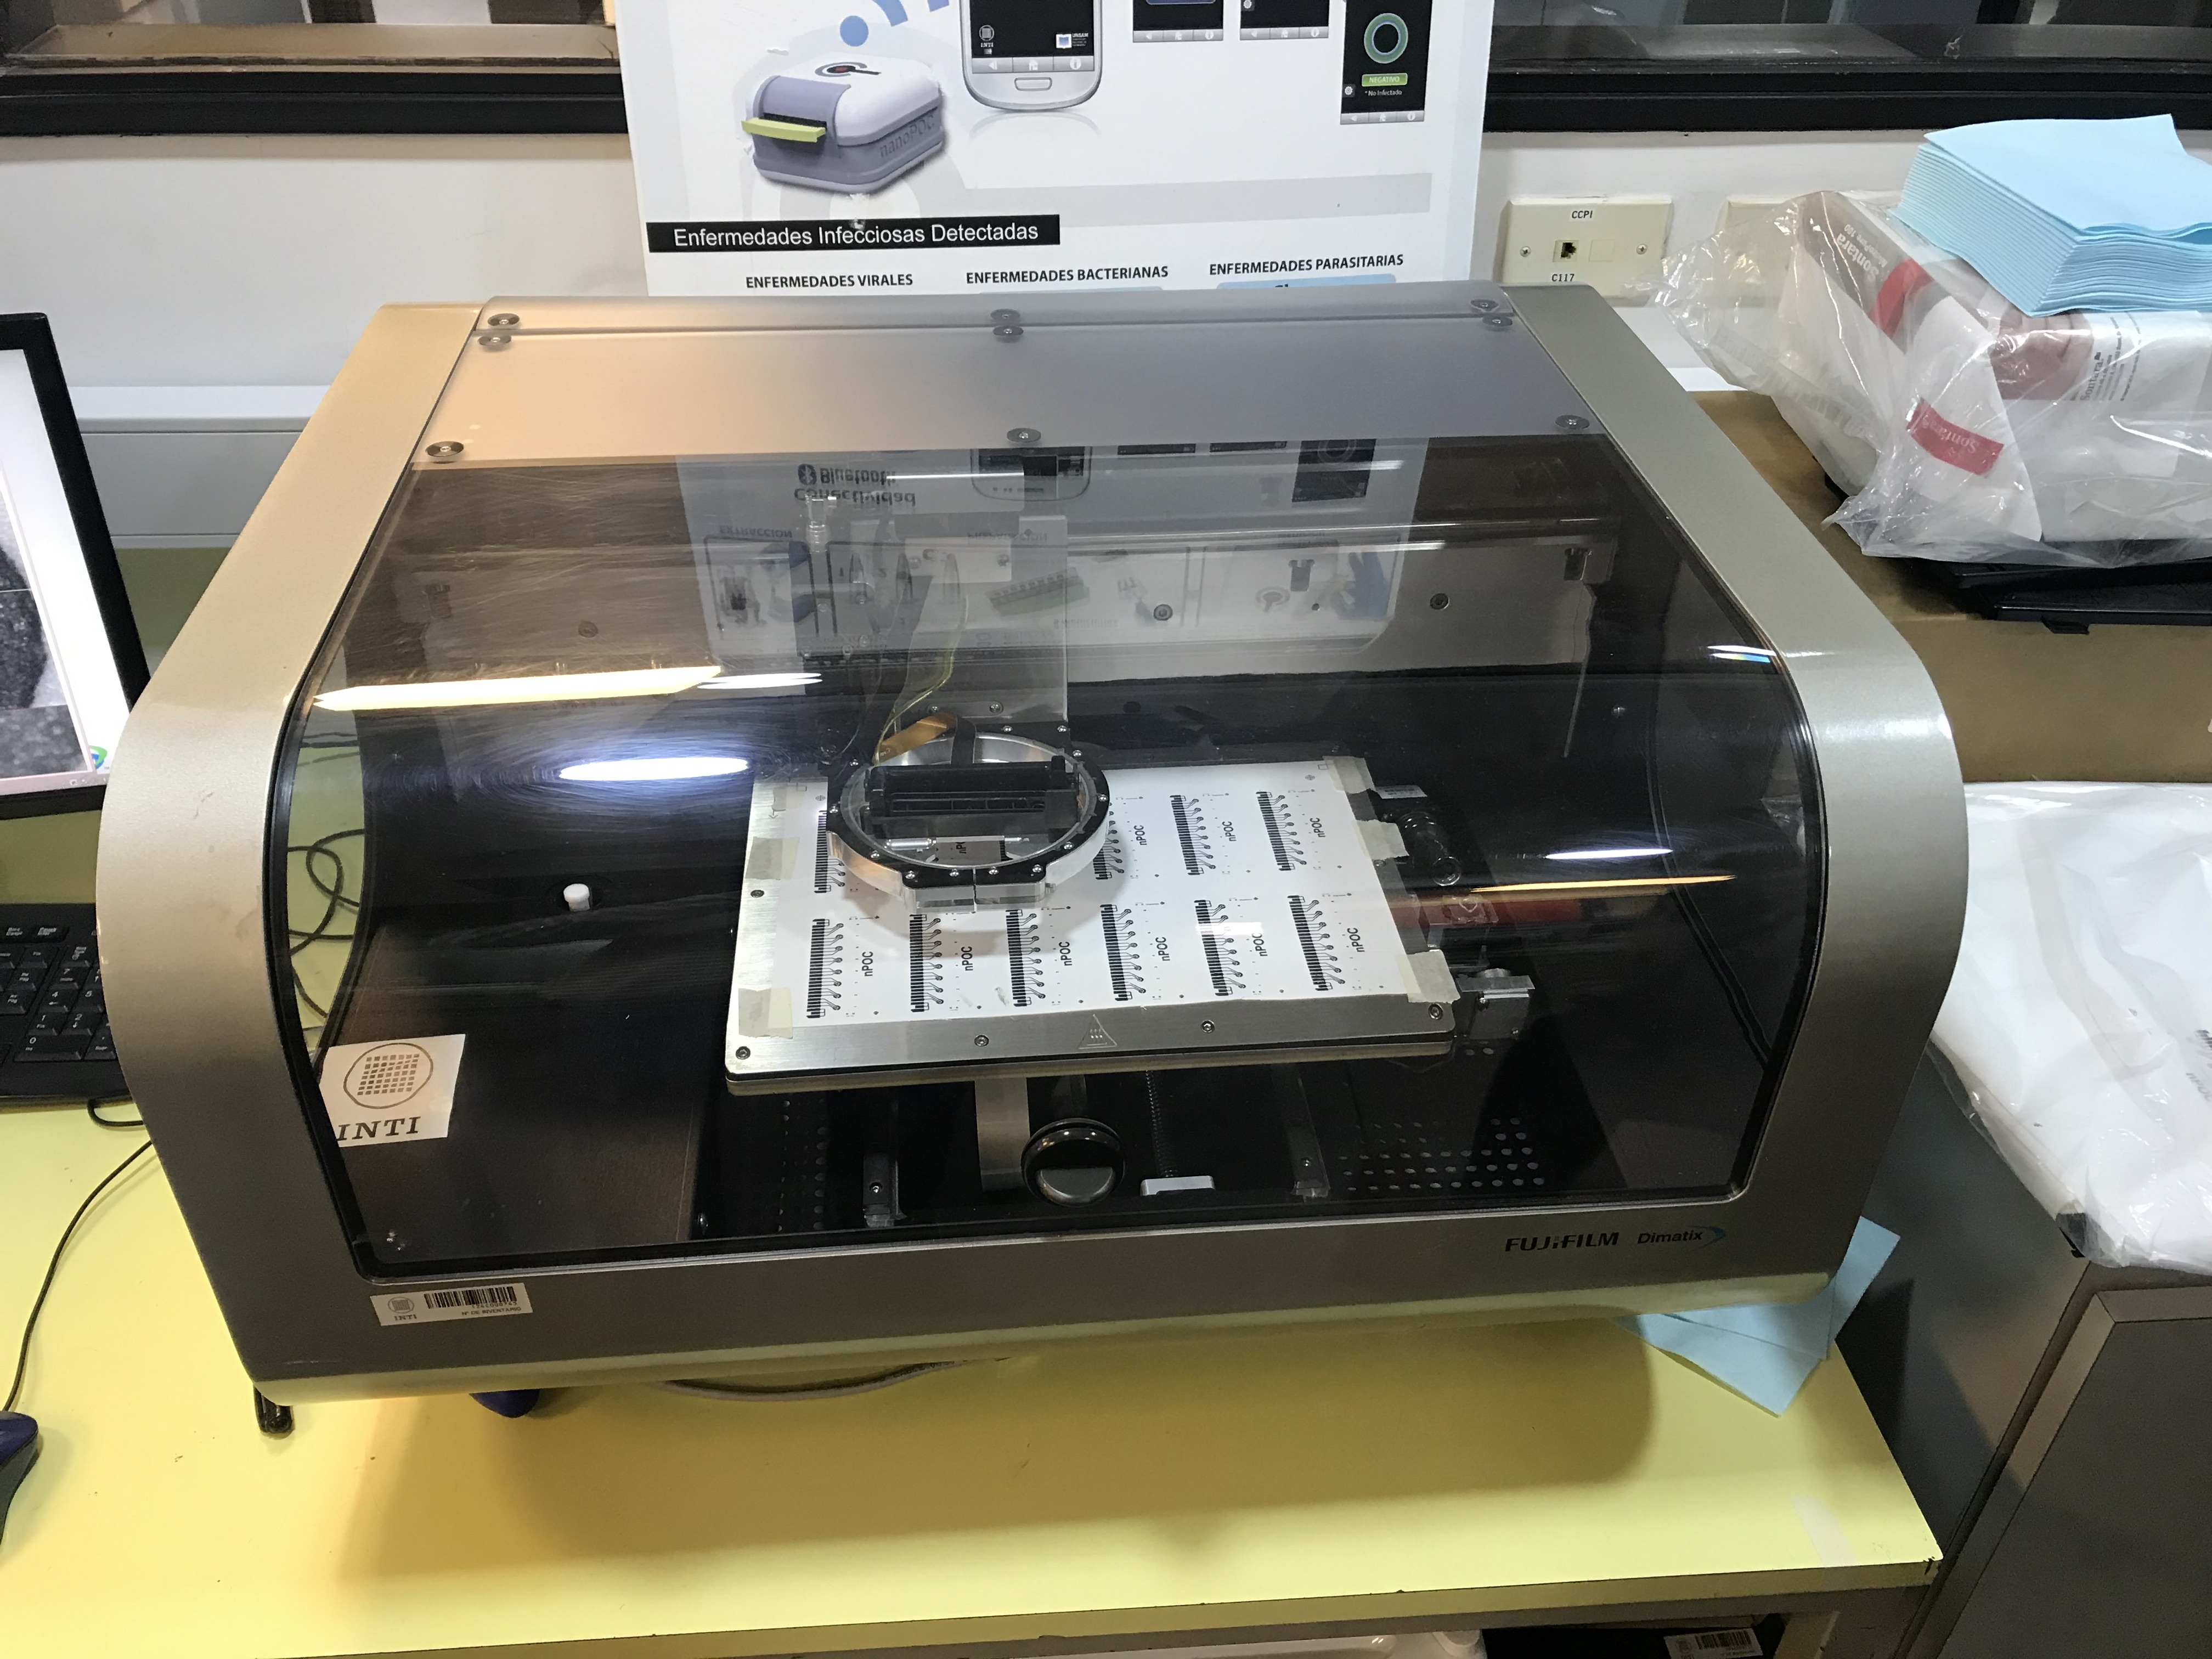
\includegraphics[width=0.5\textwidth]{Figuras/Figura_Impresora_DMP2850}
  \caption{Impresora Fujifilm Dimatix DMP-2850.}
  \label{fig:Figura_Impresora_DMP2850}
\end{figure}

El sistema de acarreo del cabezal de impresión posee un sistema para variar el ángulo del cartucho de tinta y asi modificar la distancia entre gotas de los distintos eyectores (Figura ~\ref{fig:Figura_Carriage_angulo}) y una cámara fiducial, que permite ver el sustrato y la impresión en tiempo real y realizar mediciones a través del Software incluído con la impresora (Figura ~\ref{fig:Figura_Vista_Camara_Fiducial}). 

\begin{figure}[H]
  \centering
    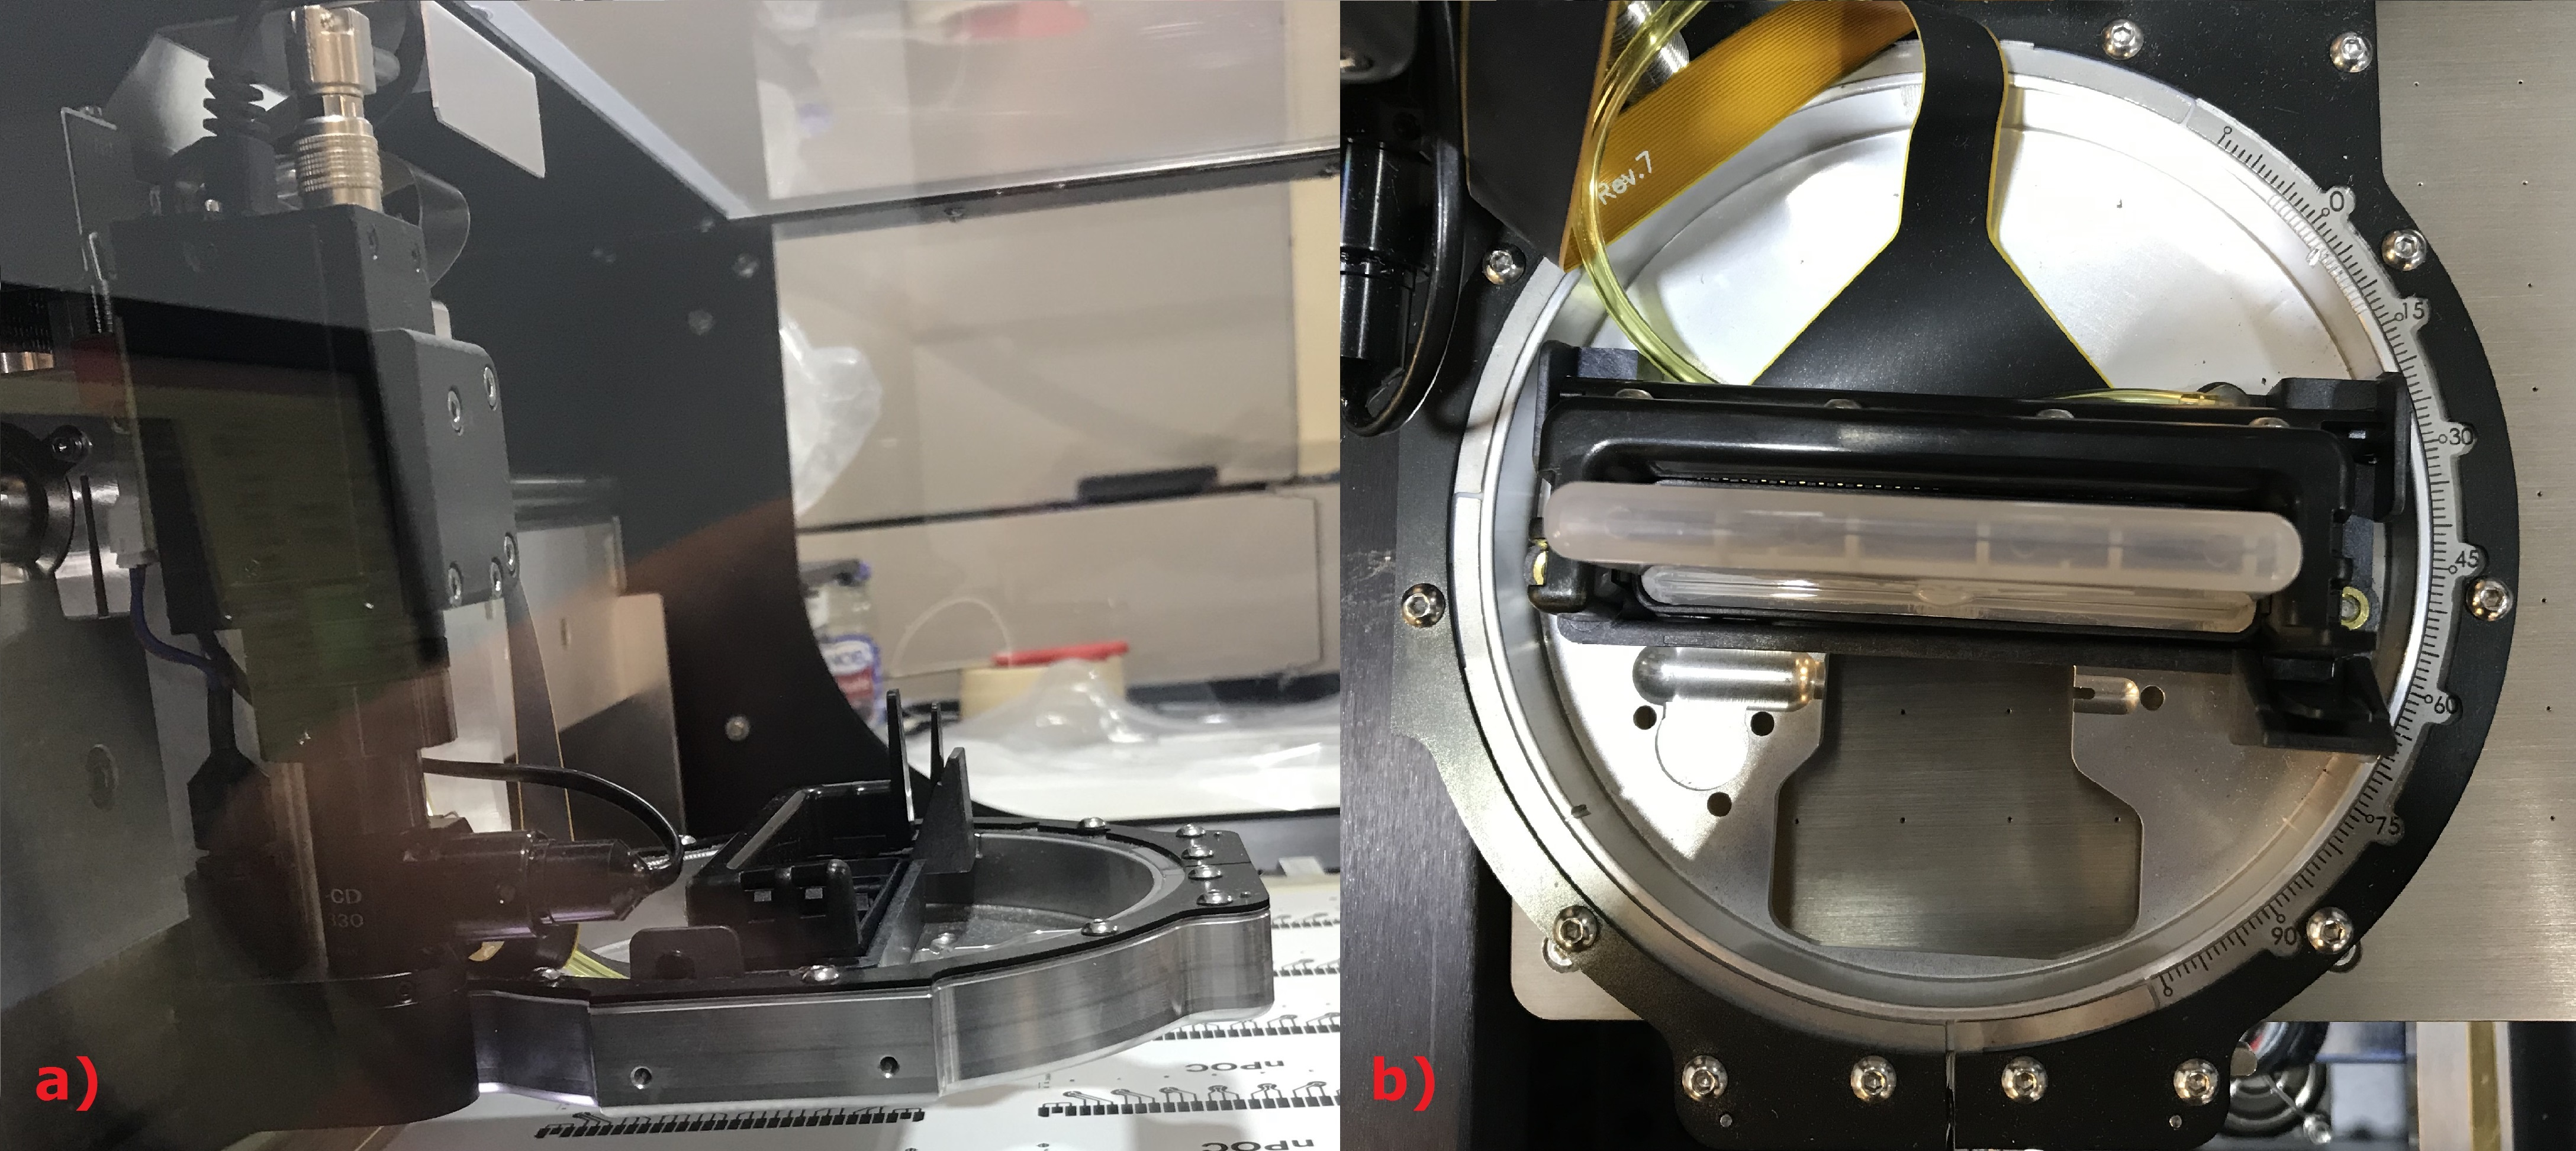
\includegraphics[width=0.8\textwidth]{Figuras/Figura_Carriage_angulo}
  \caption{a) Sistema de acarreo de cabezal de impresi\'on b) Sistema para variar el ángulo del cartucho.}
  \label{fig:Figura_Carriage_angulo}
\end{figure}

\begin{figure}[H]
  \centering
    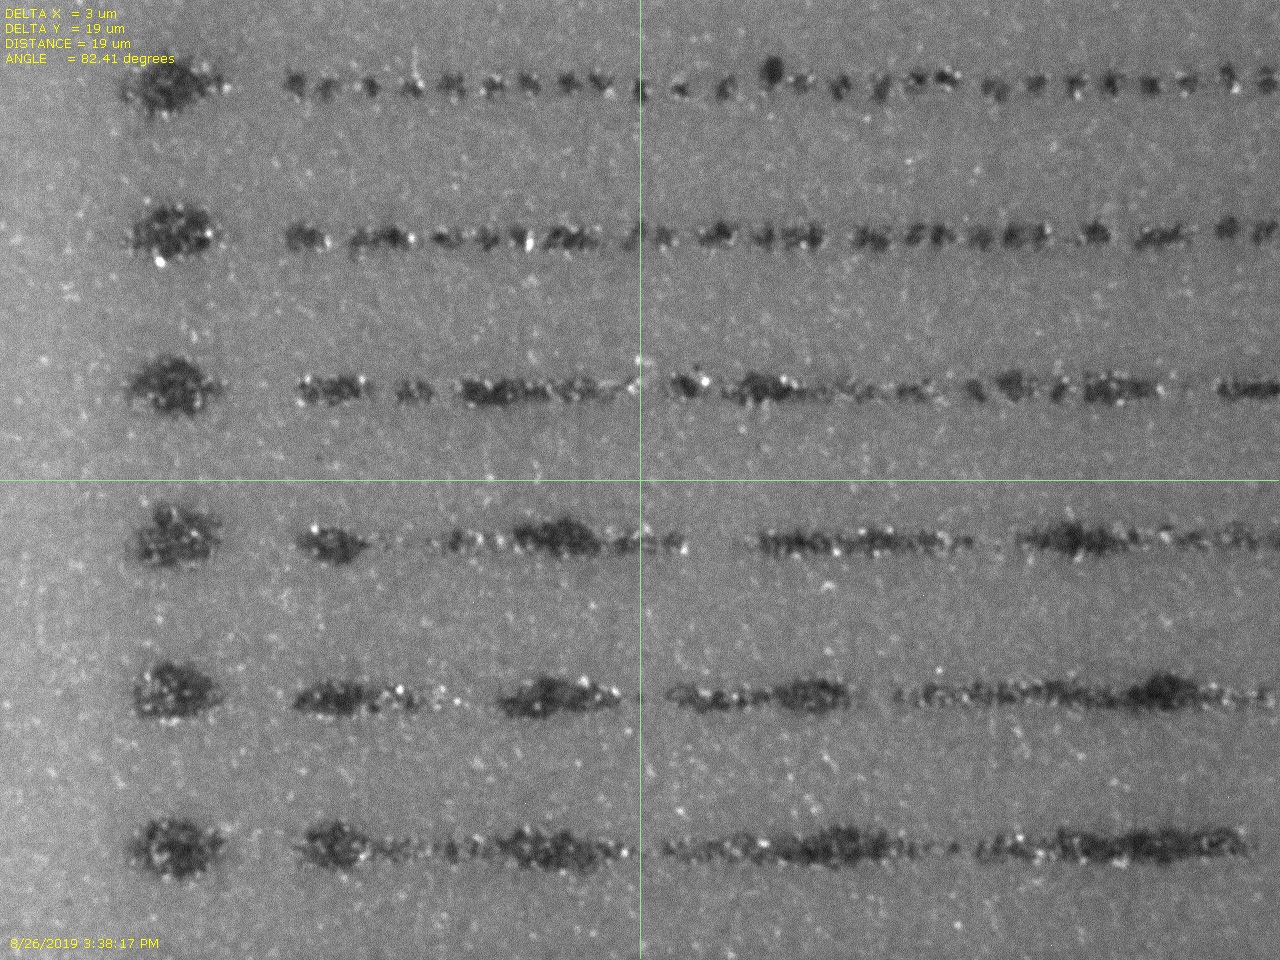
\includegraphics[width=0.5\textwidth]{Figuras/Figura_Vista_Camara_Fiducial}
  \caption{Vista de Cámara Fiducial desde Software DMP.}
  \label{fig:Figura_Vista_Camara_Fiducial}
\end{figure}

Para observar el estado del cabezal, la eyección de las gotas y calibrar el sistema de impresión se utiliza el \textit{Drop Watcher}. Este sistema consta de una cámara orientada a 45º del plano horizontal, con foco en los eyectores del cabezal (Figura ~\ref{fig:Figura_Drop_Watcher}). Mediante una luz estroboscópica se pueden realizar fotografías o filmaciones del funcionamiento de cada uno de los orificios del cabezal (Figura ~\ref{fig:Figura_Drop_Watcher}).

\begin{figure}[H]
  \centering
    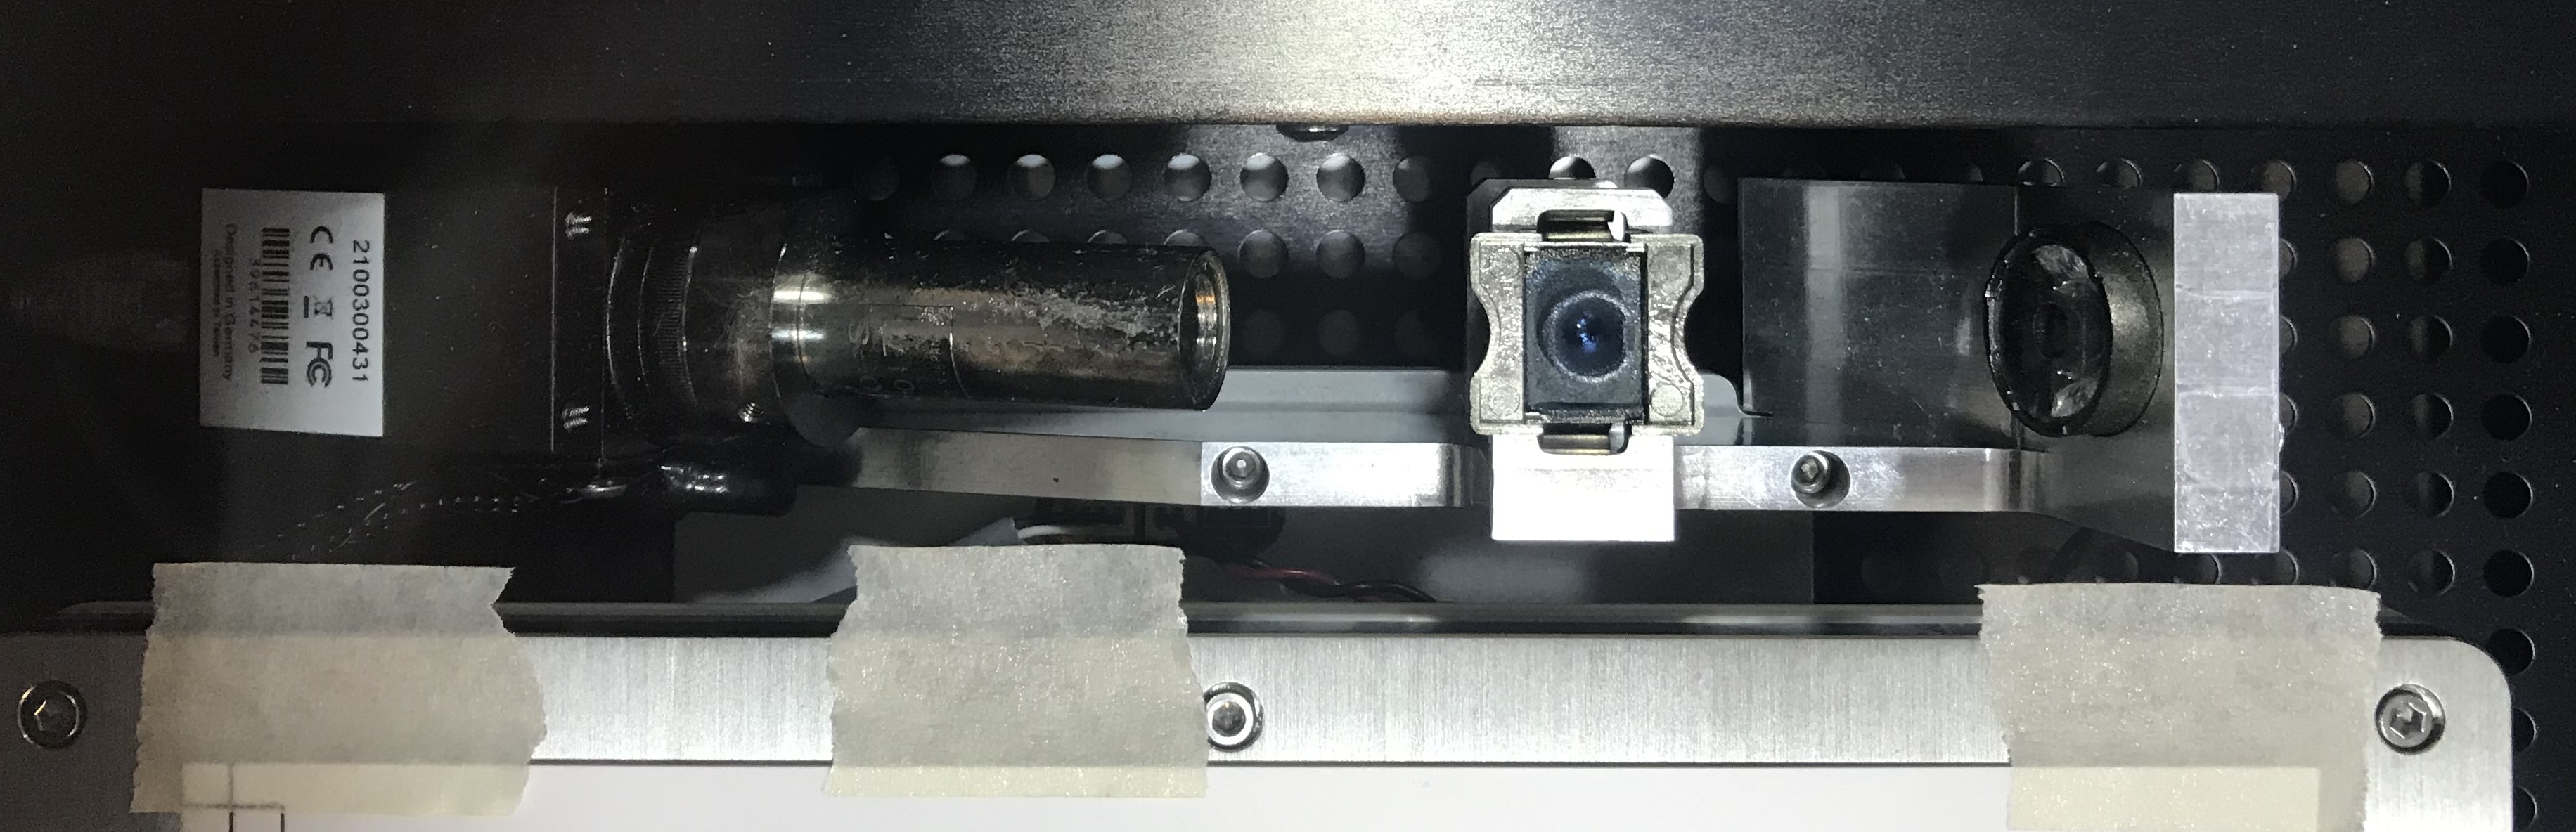
\includegraphics[width=0.5\textwidth]{Figuras/Figura_Camara_Drop_Watcher}
  \caption{Sistema de cámara, luz y reservorio de \textit{Drop Watcher}.}
  \label{fig:Figura_Camara_Drop_Watcher}
\end{figure}

\begin{figure}[H]
  \centering
    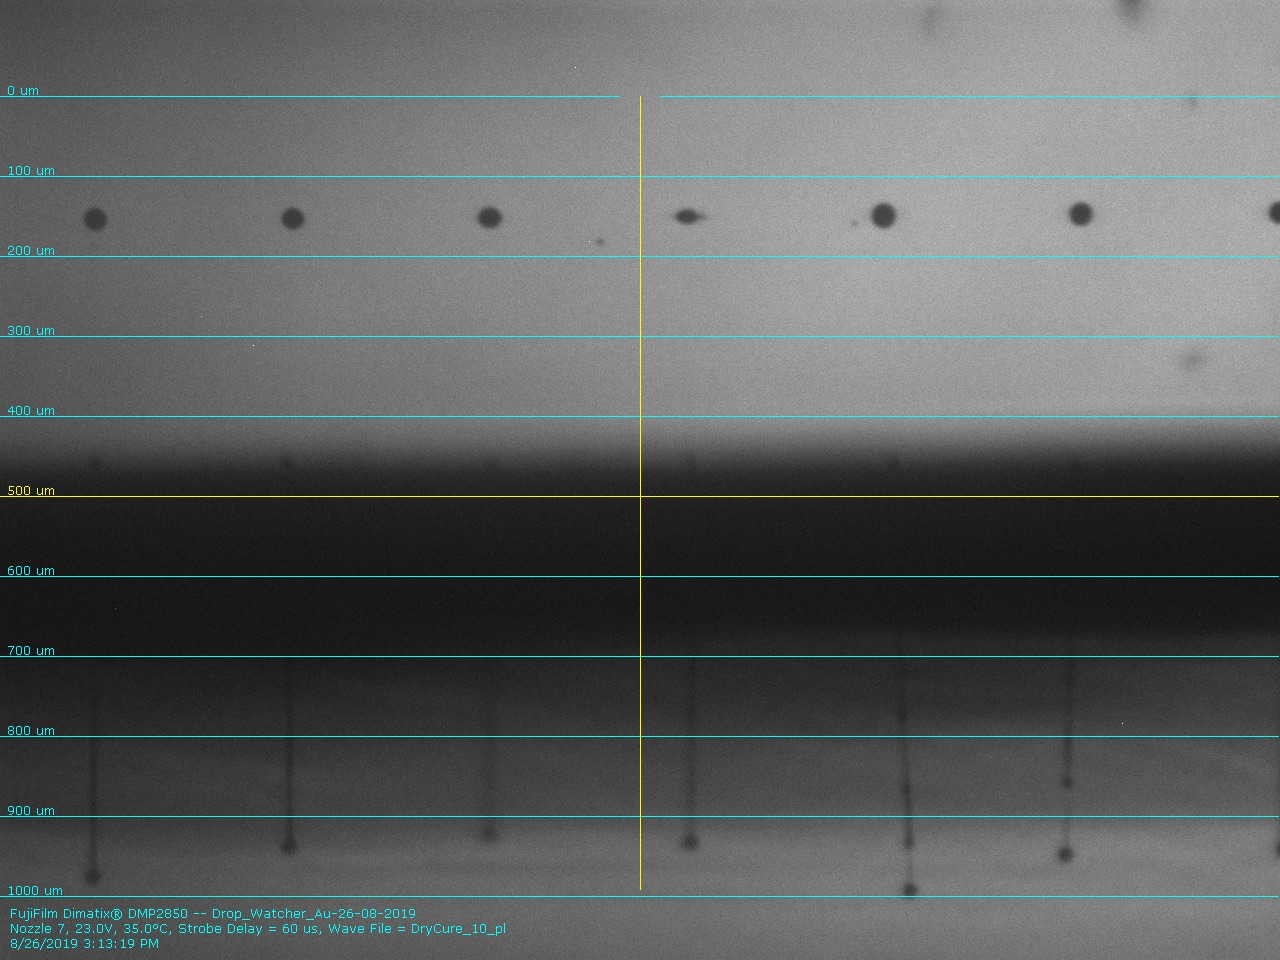
\includegraphics[width=0.5\textwidth]{Figuras/Figura_Drop_Watcher}
  \caption{Imágen de gotas siendo eyectadas mediante Software DMP.}
  \label{fig:Figura_Drop_Watcher}
\end{figure}

\section{Preparación de cartucho de tinta}
Dado que los reservorios y cabezales solo pueden utilizarse con un tipo de tinta, Fujifilm los ofrece en forma de Kits para impresión (Figura ~\ref{fig:Figura_kit_impresion}). Cada Kit consta de un reservorio de 3 ml, un cabezal (dependiendo del modelo puede ser de 1 pl o 10 pl, haciendo referencia al volumen de la gota eyectada), una jeringa de 3 ml, una aguja de punta redonda y un $``$\textit{pad}$"$ de limpieza (Figura ~\ref{fig:Figura_Cleaning_pad}). El tamaño de la jeringa no permite que se deposite un volumen mayor de tinta al soportado por el sistema del reservorio. El largo de la aguja previene la rotura del contenedor del cartucho.

\begin{figure}[H]
  \centering
    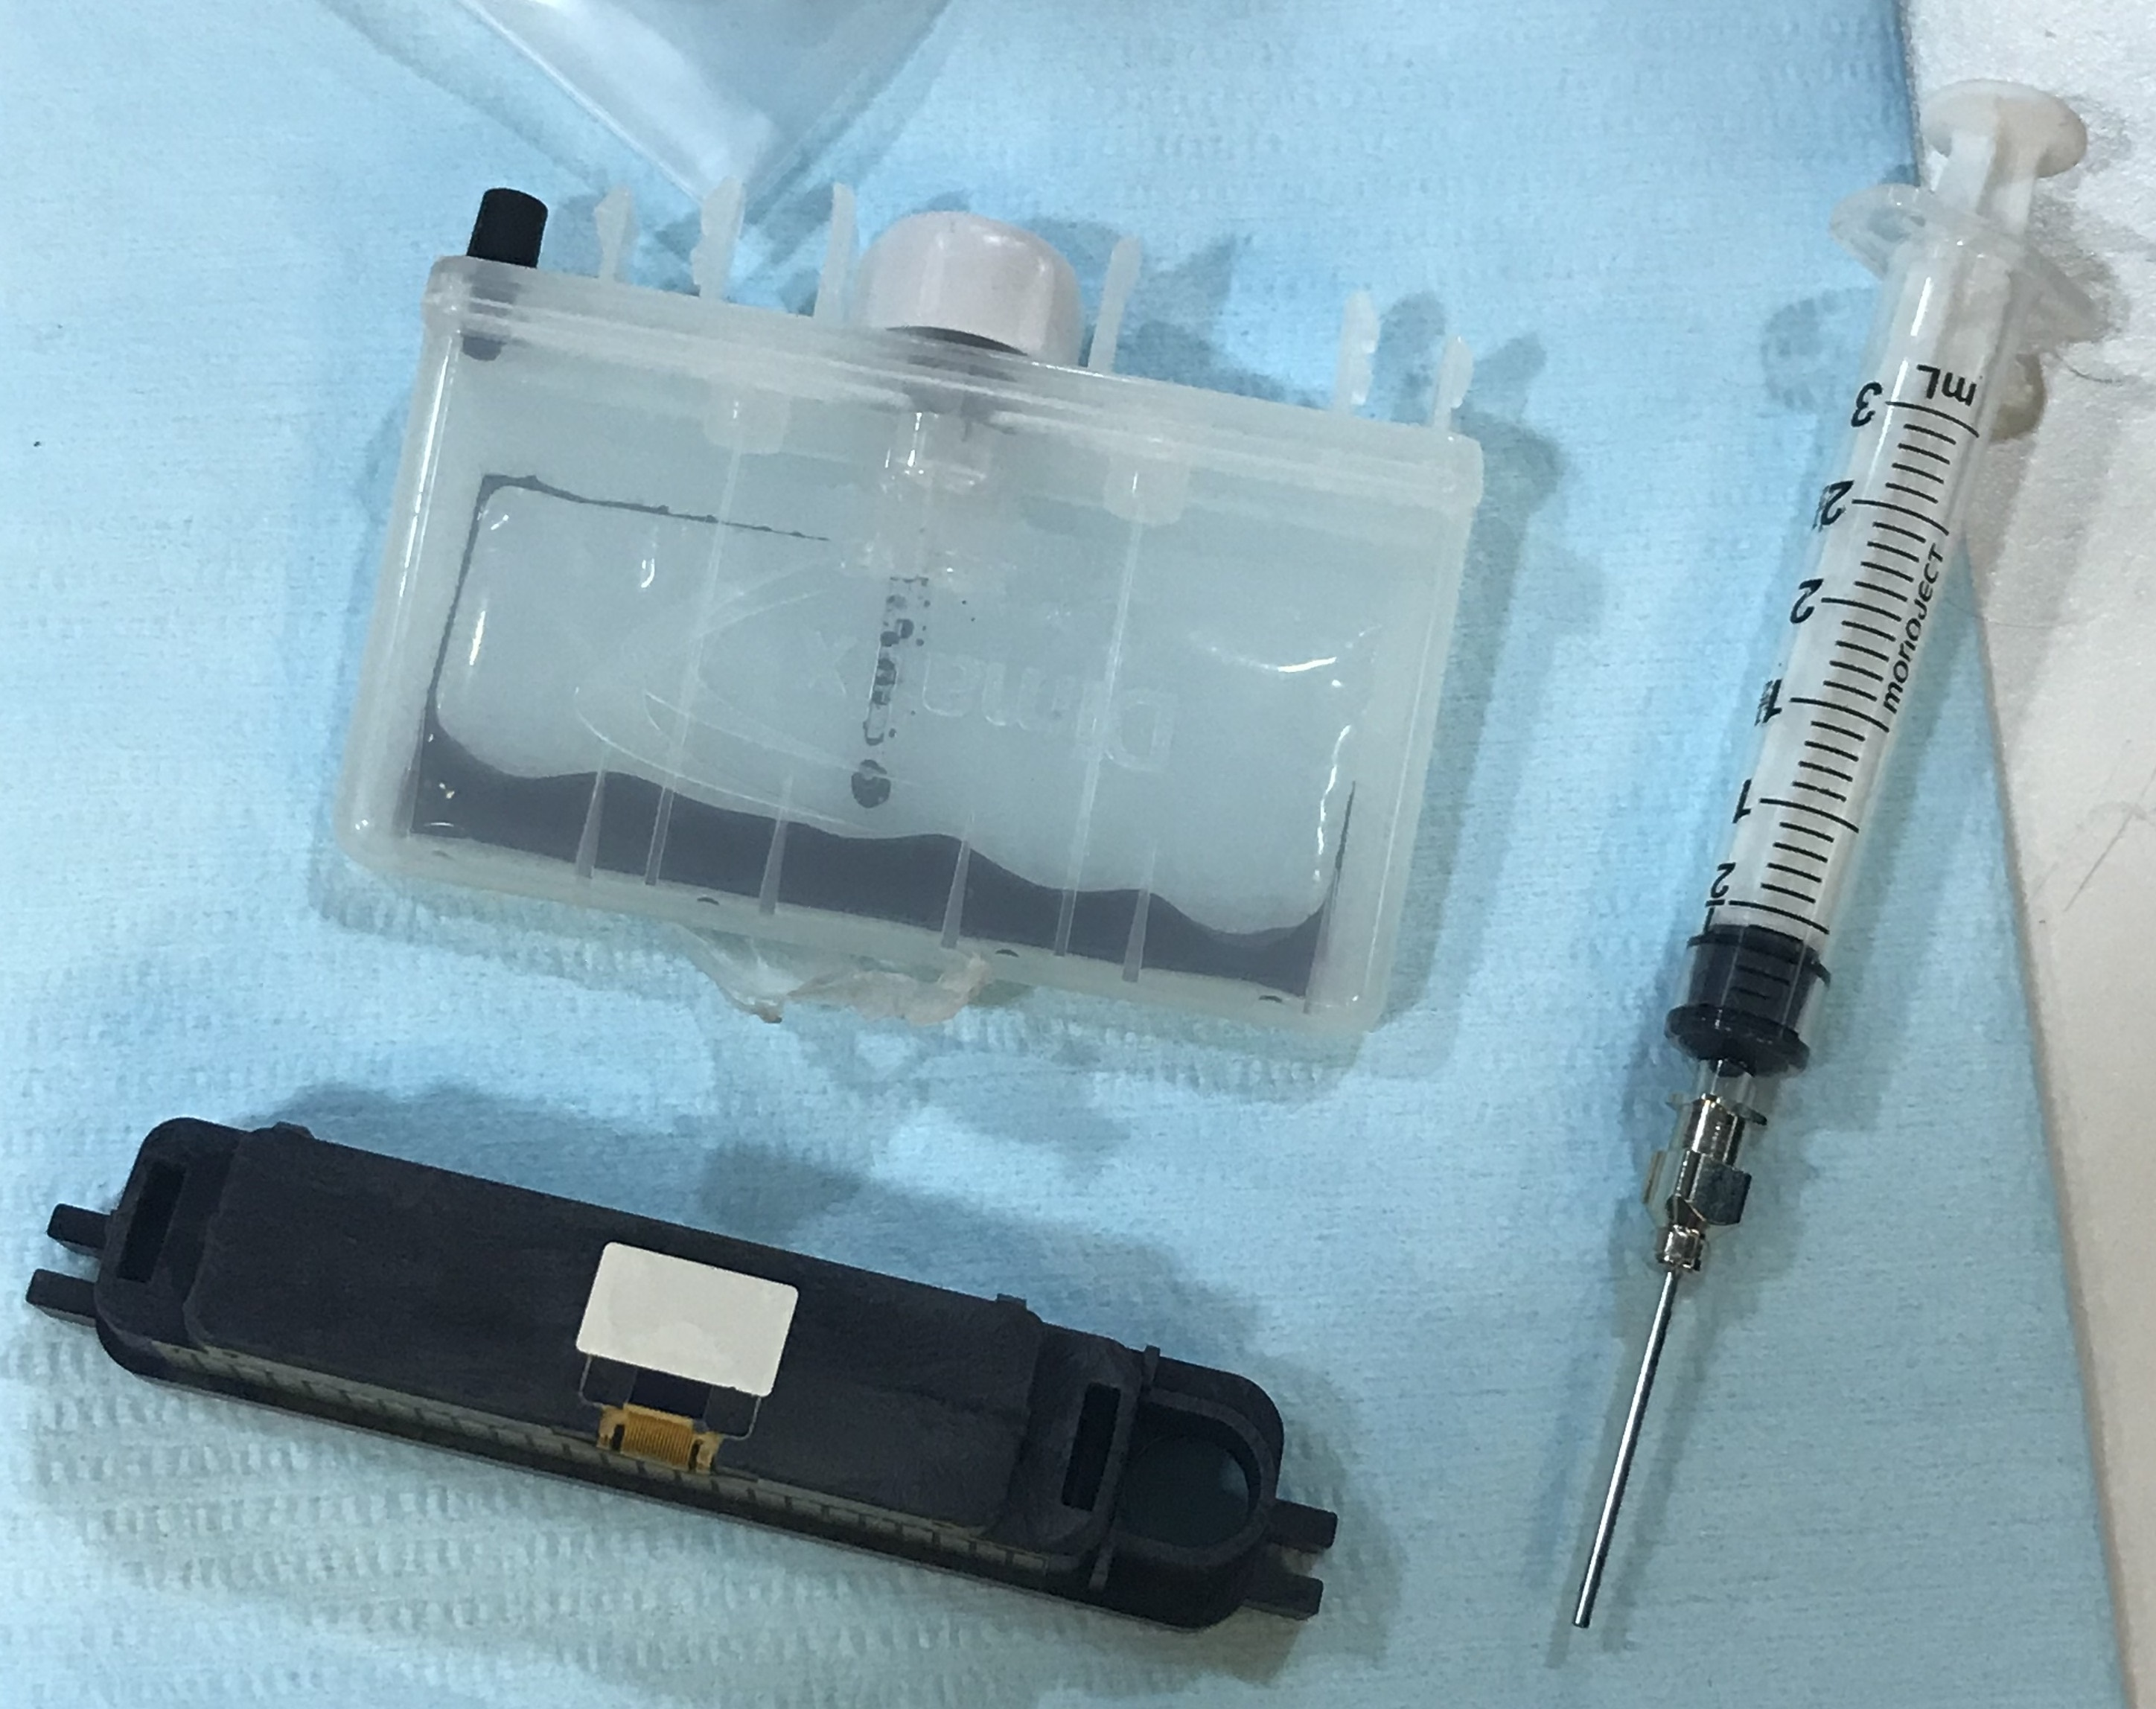
\includegraphics[width=0.5\textwidth]{Figuras/Figura_kit_impresion}
  \caption{Kit de impresión para Fujifilm Dimatix DMP2850 con cabezal de 10 pl lleno de tinta de nanopartículas de oro.}
  \label{fig:Figura_kit_impresion}
\end{figure}

\begin{figure}[H]
  \centering
    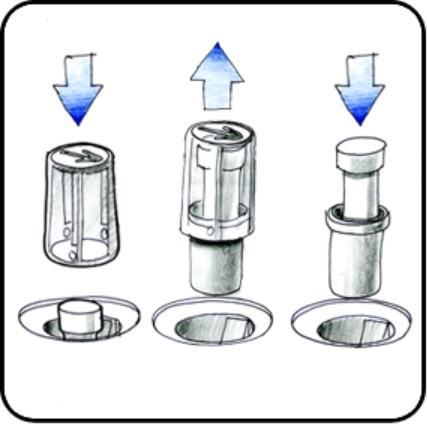
\includegraphics[width=0.5\textwidth]{Figuras/Figura_Cleaning_pad}
  \caption{Modo de uso de \textit{Cleaning Pad}.}
  \label{fig:Figura_Cleaning_pad}
\end{figure}

El $``$\textit{pad}$"$ de limpieza (\textit{Cleaning Pad} en inglés) se debe reemplazar una vez que se haya saturado de tinta. Esto se notará por un exceso de material sobre el sustrato, el taponamiento de eyectores o irregularidades en la impresión, como un mal alineamiento de las gotas sobre el sustrato. Para comprobar si se trata de tinta depositada sobre el cabezal se utiliza el \textit{Drop Watcher}, donde puede verse fácilmente el estado de los eyectores y el vuelo de las gotas. (Figura ~\ref{fig:Figura_suciedad_cabezal}).

\begin{figure}[H]
  \centering
    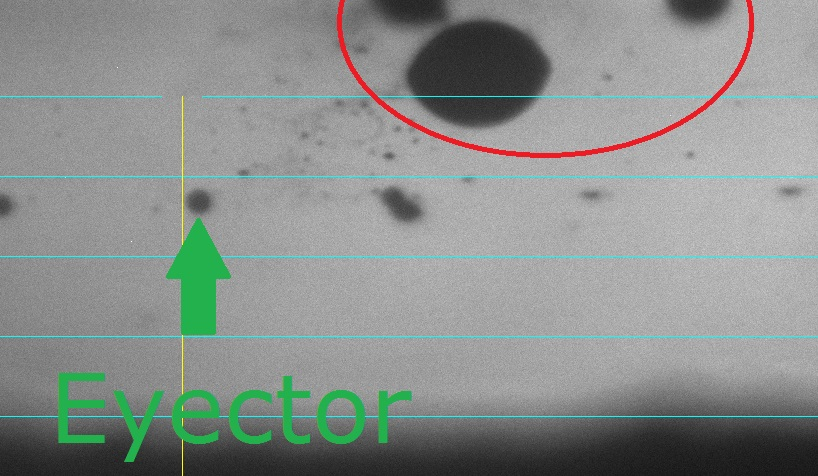
\includegraphics[width=0.5\textwidth]{Figuras/Figura_suciedad_cabezal}
  \caption{Tinta depositada sobre cabezal por $``$\textit{pad}$"$ de limpieza saturado.}
  \label{fig:Figura_suciedad_cabezal}
\end{figure}

En primera instancia se toma la cantidad de tinta a utilizar con la jeringa y se deposita dentro del reservorio. El largo de la aguja no permite llegar hasta el final del reservorio, preveniendo la perforación del mismo (Figura ~\ref{fig:Figura_carga_tinta}).

\begin{figure}[H]
  \centering
    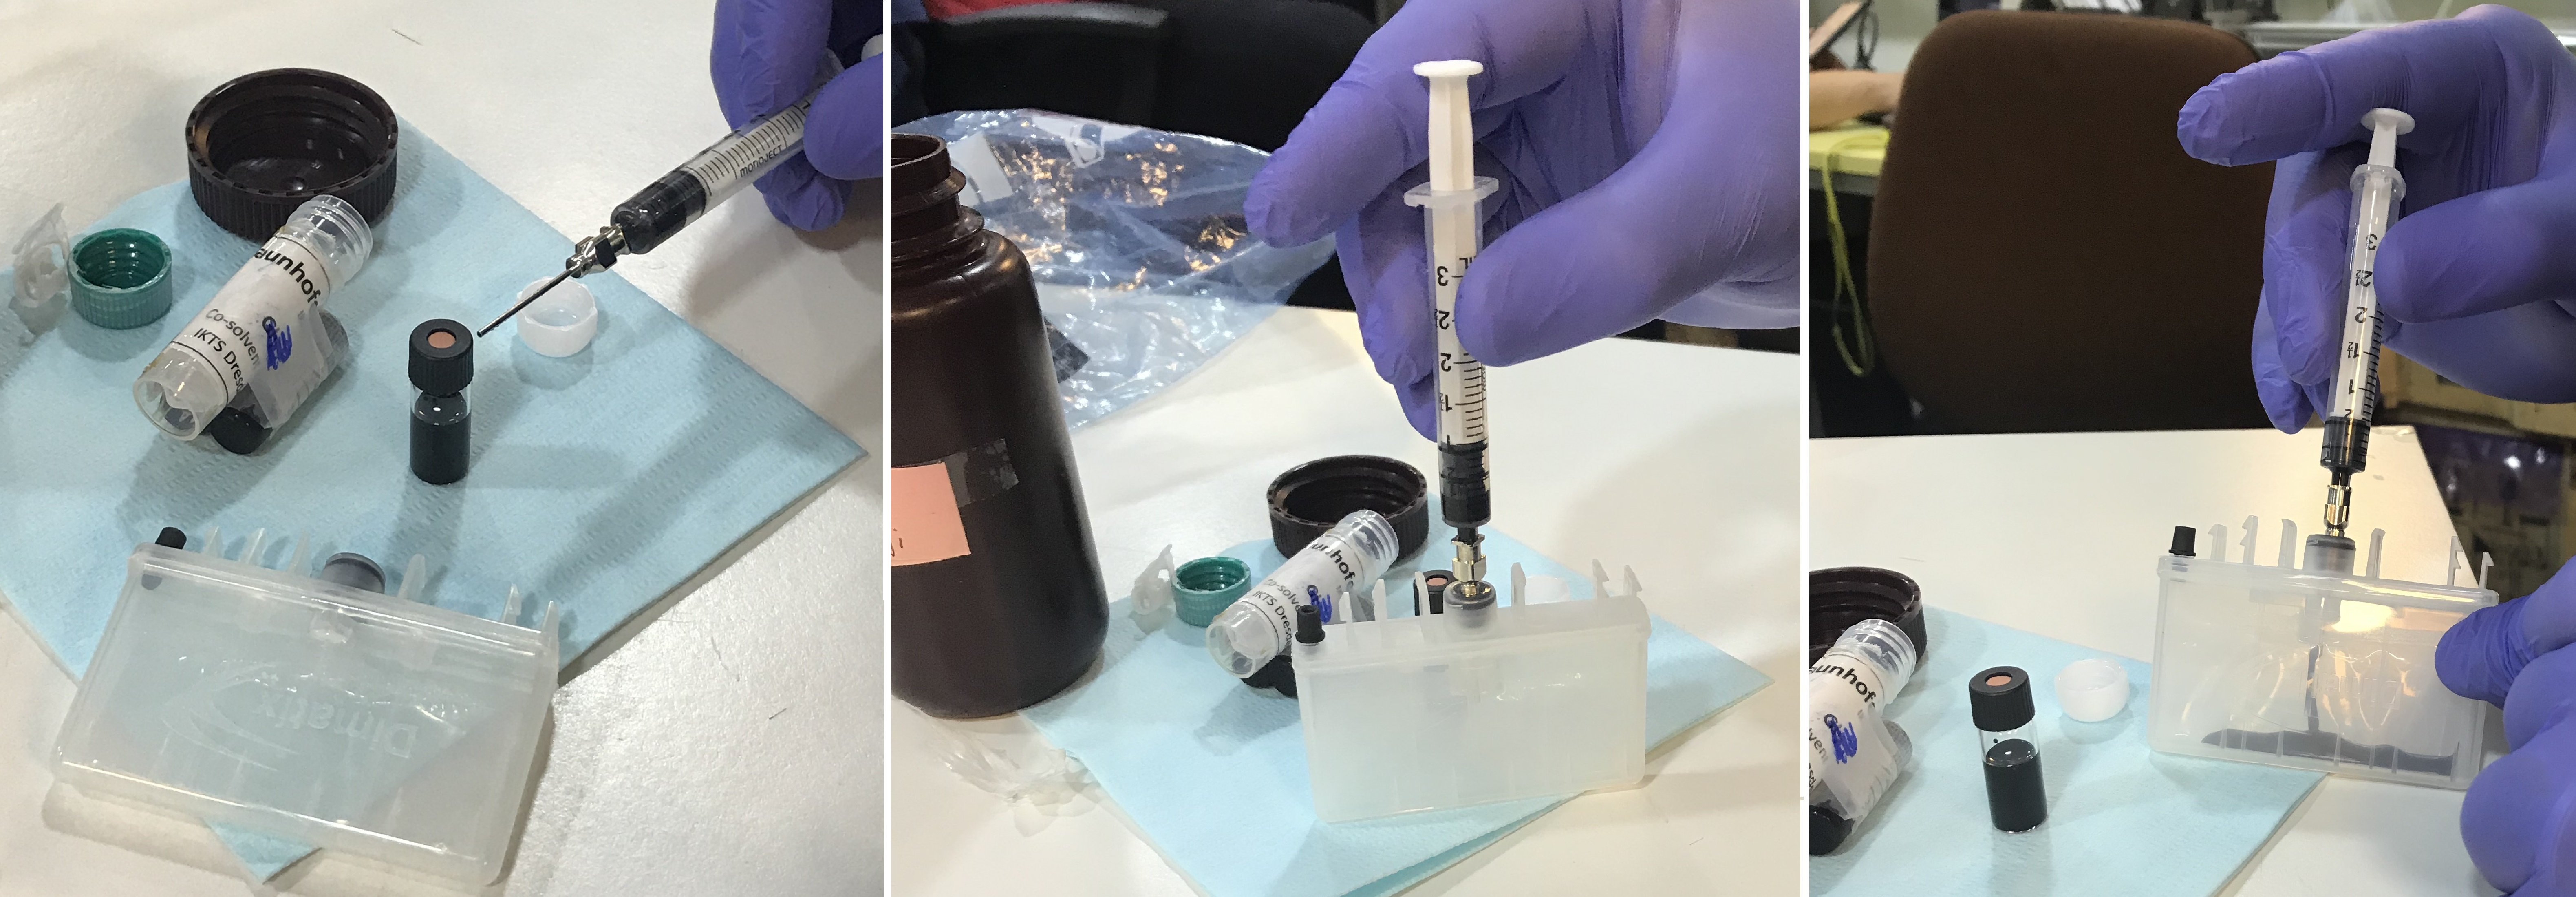
\includegraphics[width=1\textwidth]{Figuras/Figura_carga_tinta}
  \caption{Procedimiento de llenado de reservorio.}
  \label{fig:Figura_carga_tinta}
\end{figure}

Una vez que se llenó el depósito con la tinta deseada, se instala el reservorio sobre el cabezal. Dado que el mismo tiene conexión a una línea de presión para generar vacío en el interior ayudando al movimiento de la tinta, el cartucho puede armarse solo en un sentido. Según las recomendaciones de Fujifilm, se debe ajustar primero del lado del conector de vacío, apretando hasta escuchar un $``$\textit{click}$"$, luego comprobar que el tanque de tinta se encuentra alineado con el cabezal y volver a hacer fuerza sobre el mismo hasta escuchar un segundo $``$\textit{click}$"$. De esta forma, el deposito de tinta queda anclado al cabezal.

El cartucho se debe introducir en el carrete (Figura ~\ref{fig:Figura_Carrete1}) teniendo en cuenta que la orientación correcta es la que permite que los contactos del cabezal queden alineados con los del carrete. Para esto la impresora debe estar encendida y el Software \textit{Dimatix Drop Manager} en ejecución con su procedimiento de chequeo inicial completo.

\begin{figure}[H]
  \centering
    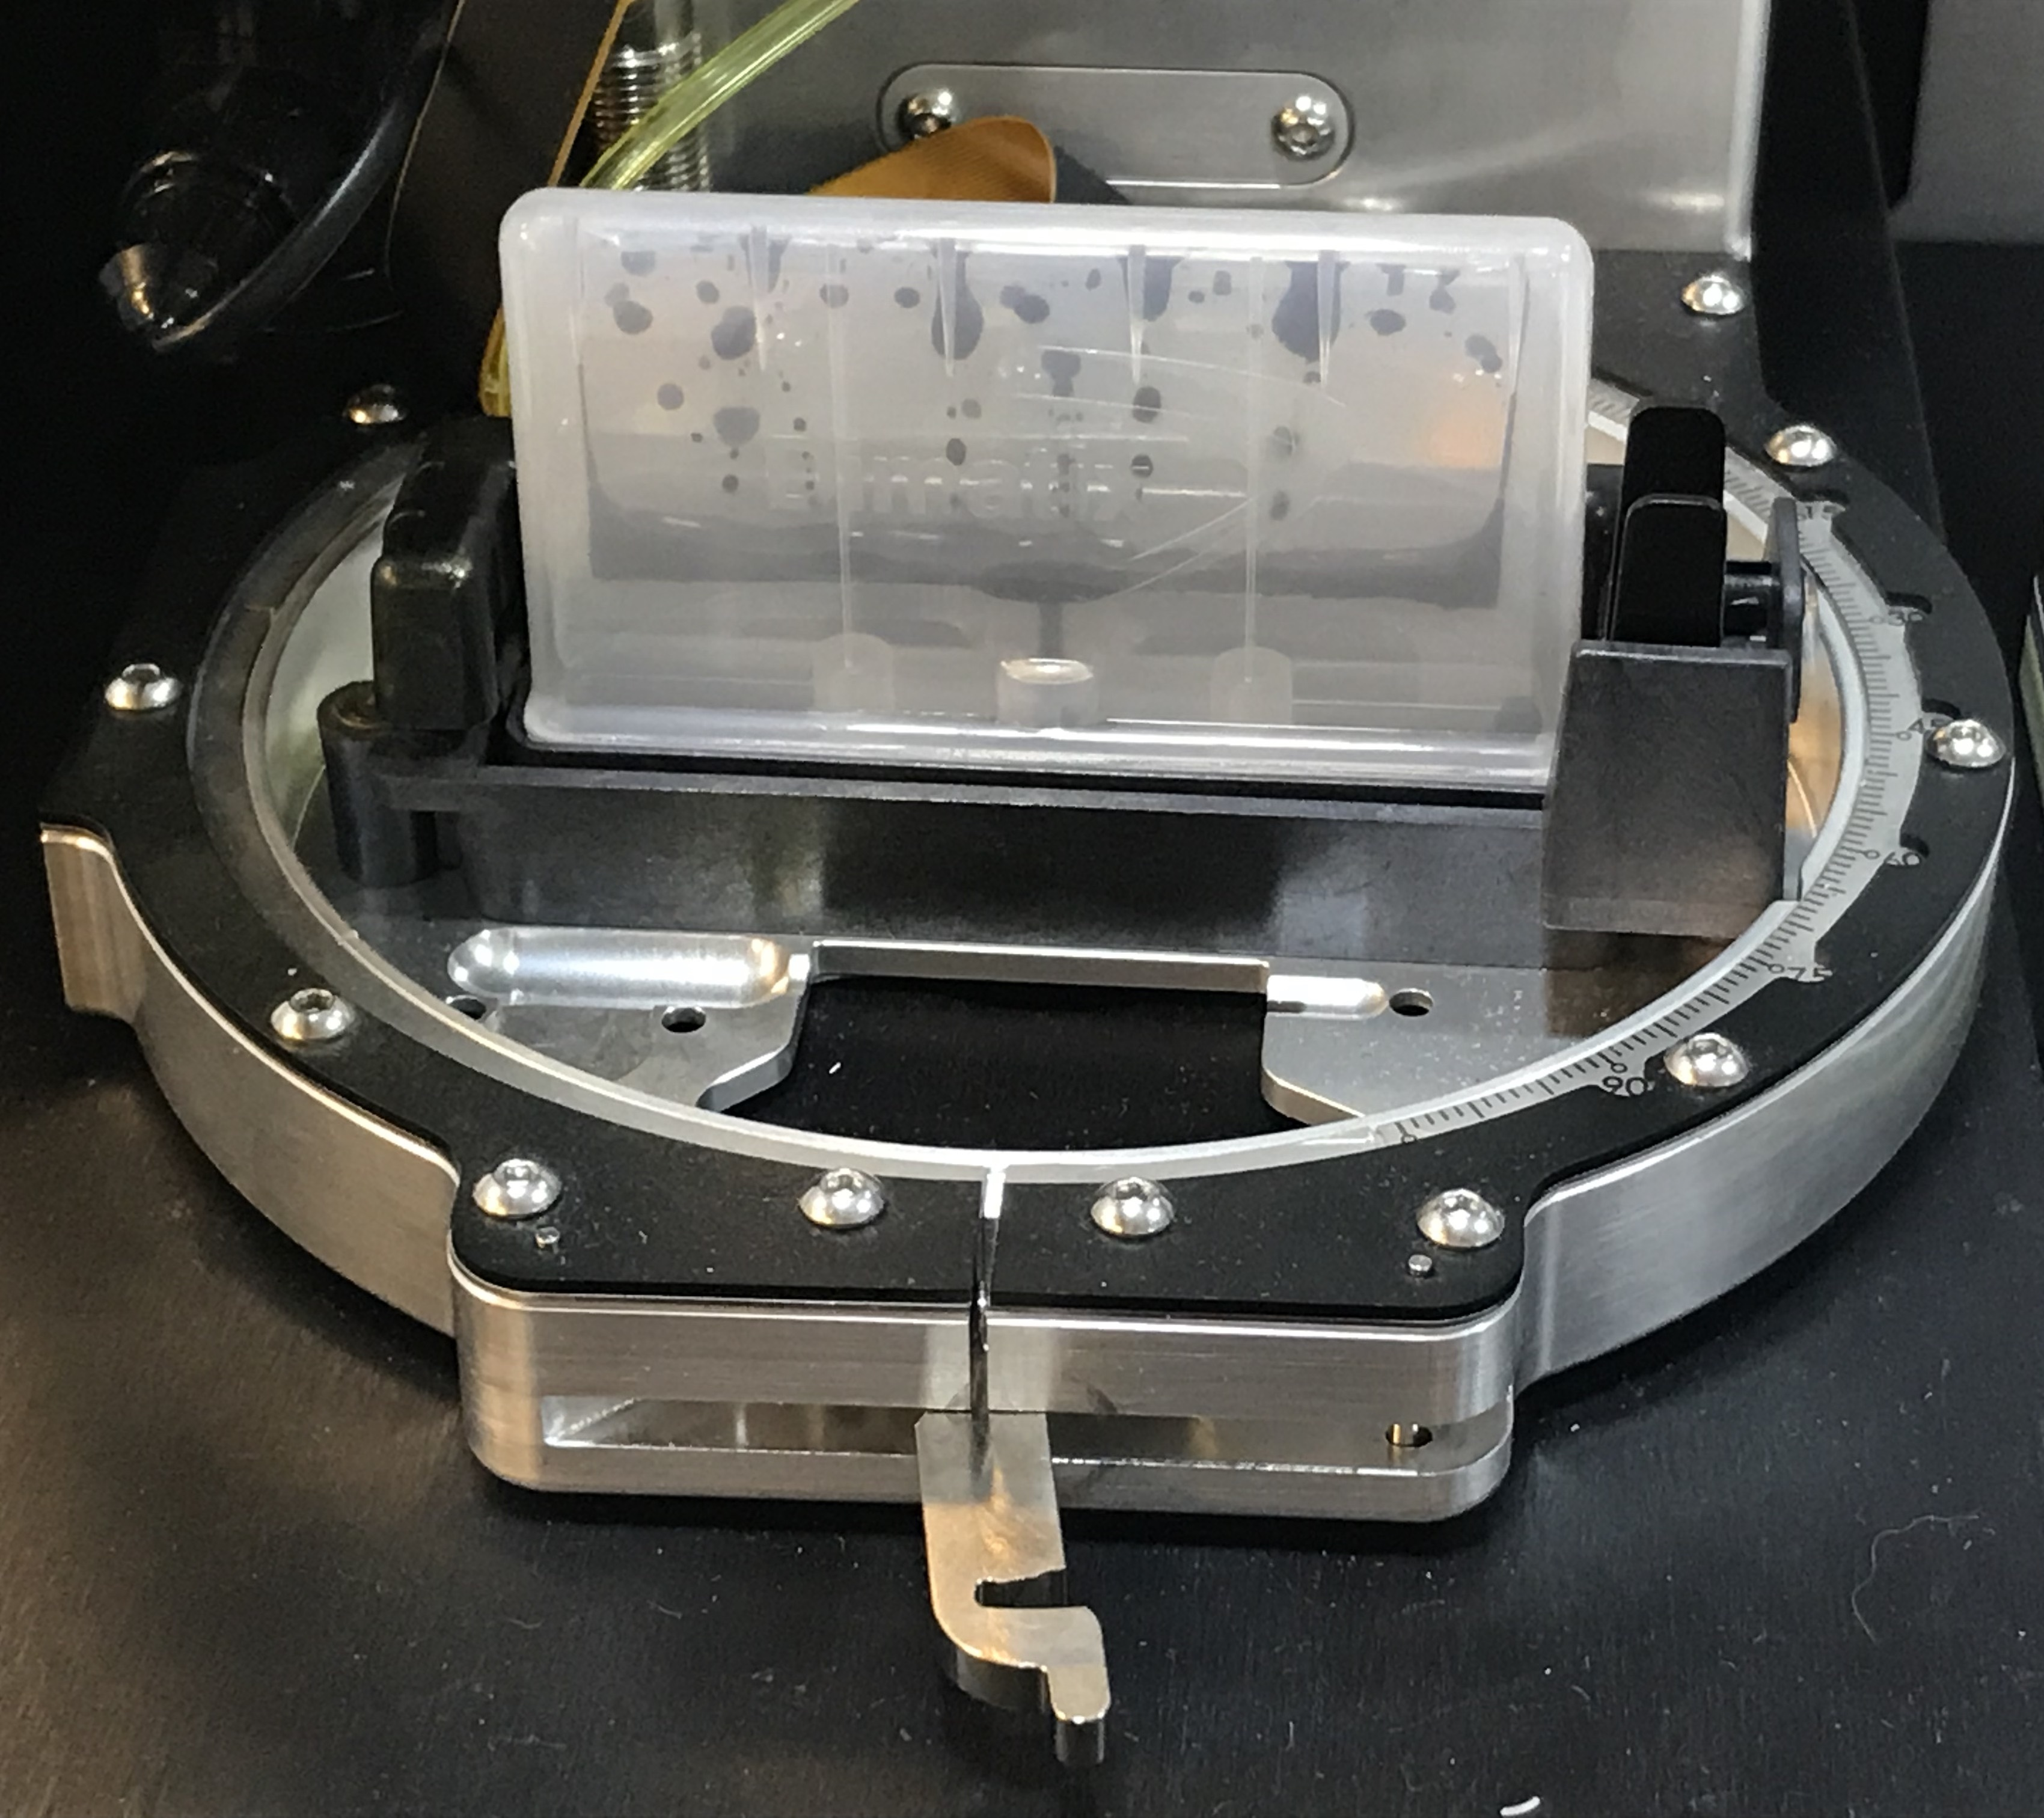
\includegraphics[width=0.5\textwidth]{Figuras/Figura_Carrete1}
  \caption{Carrete donde se instala el cartucho.}
  \label{fig:Figura_Carrete1}
\end{figure}

Una vez instalado el cartucho, se deposita el $``$\textit{pad}$"$ de limpieza en el orificio dedicado para este objeto (Figura ~\ref{fig:Figura_Orificio_Cleaning_Pad}). Esto debe hacerse antes de cerrar el procedimiento de instalación del cartucho para evitar el derrame de tinta sobre la base de descanso del carrete.

\begin{figure}[H]
  \centering
    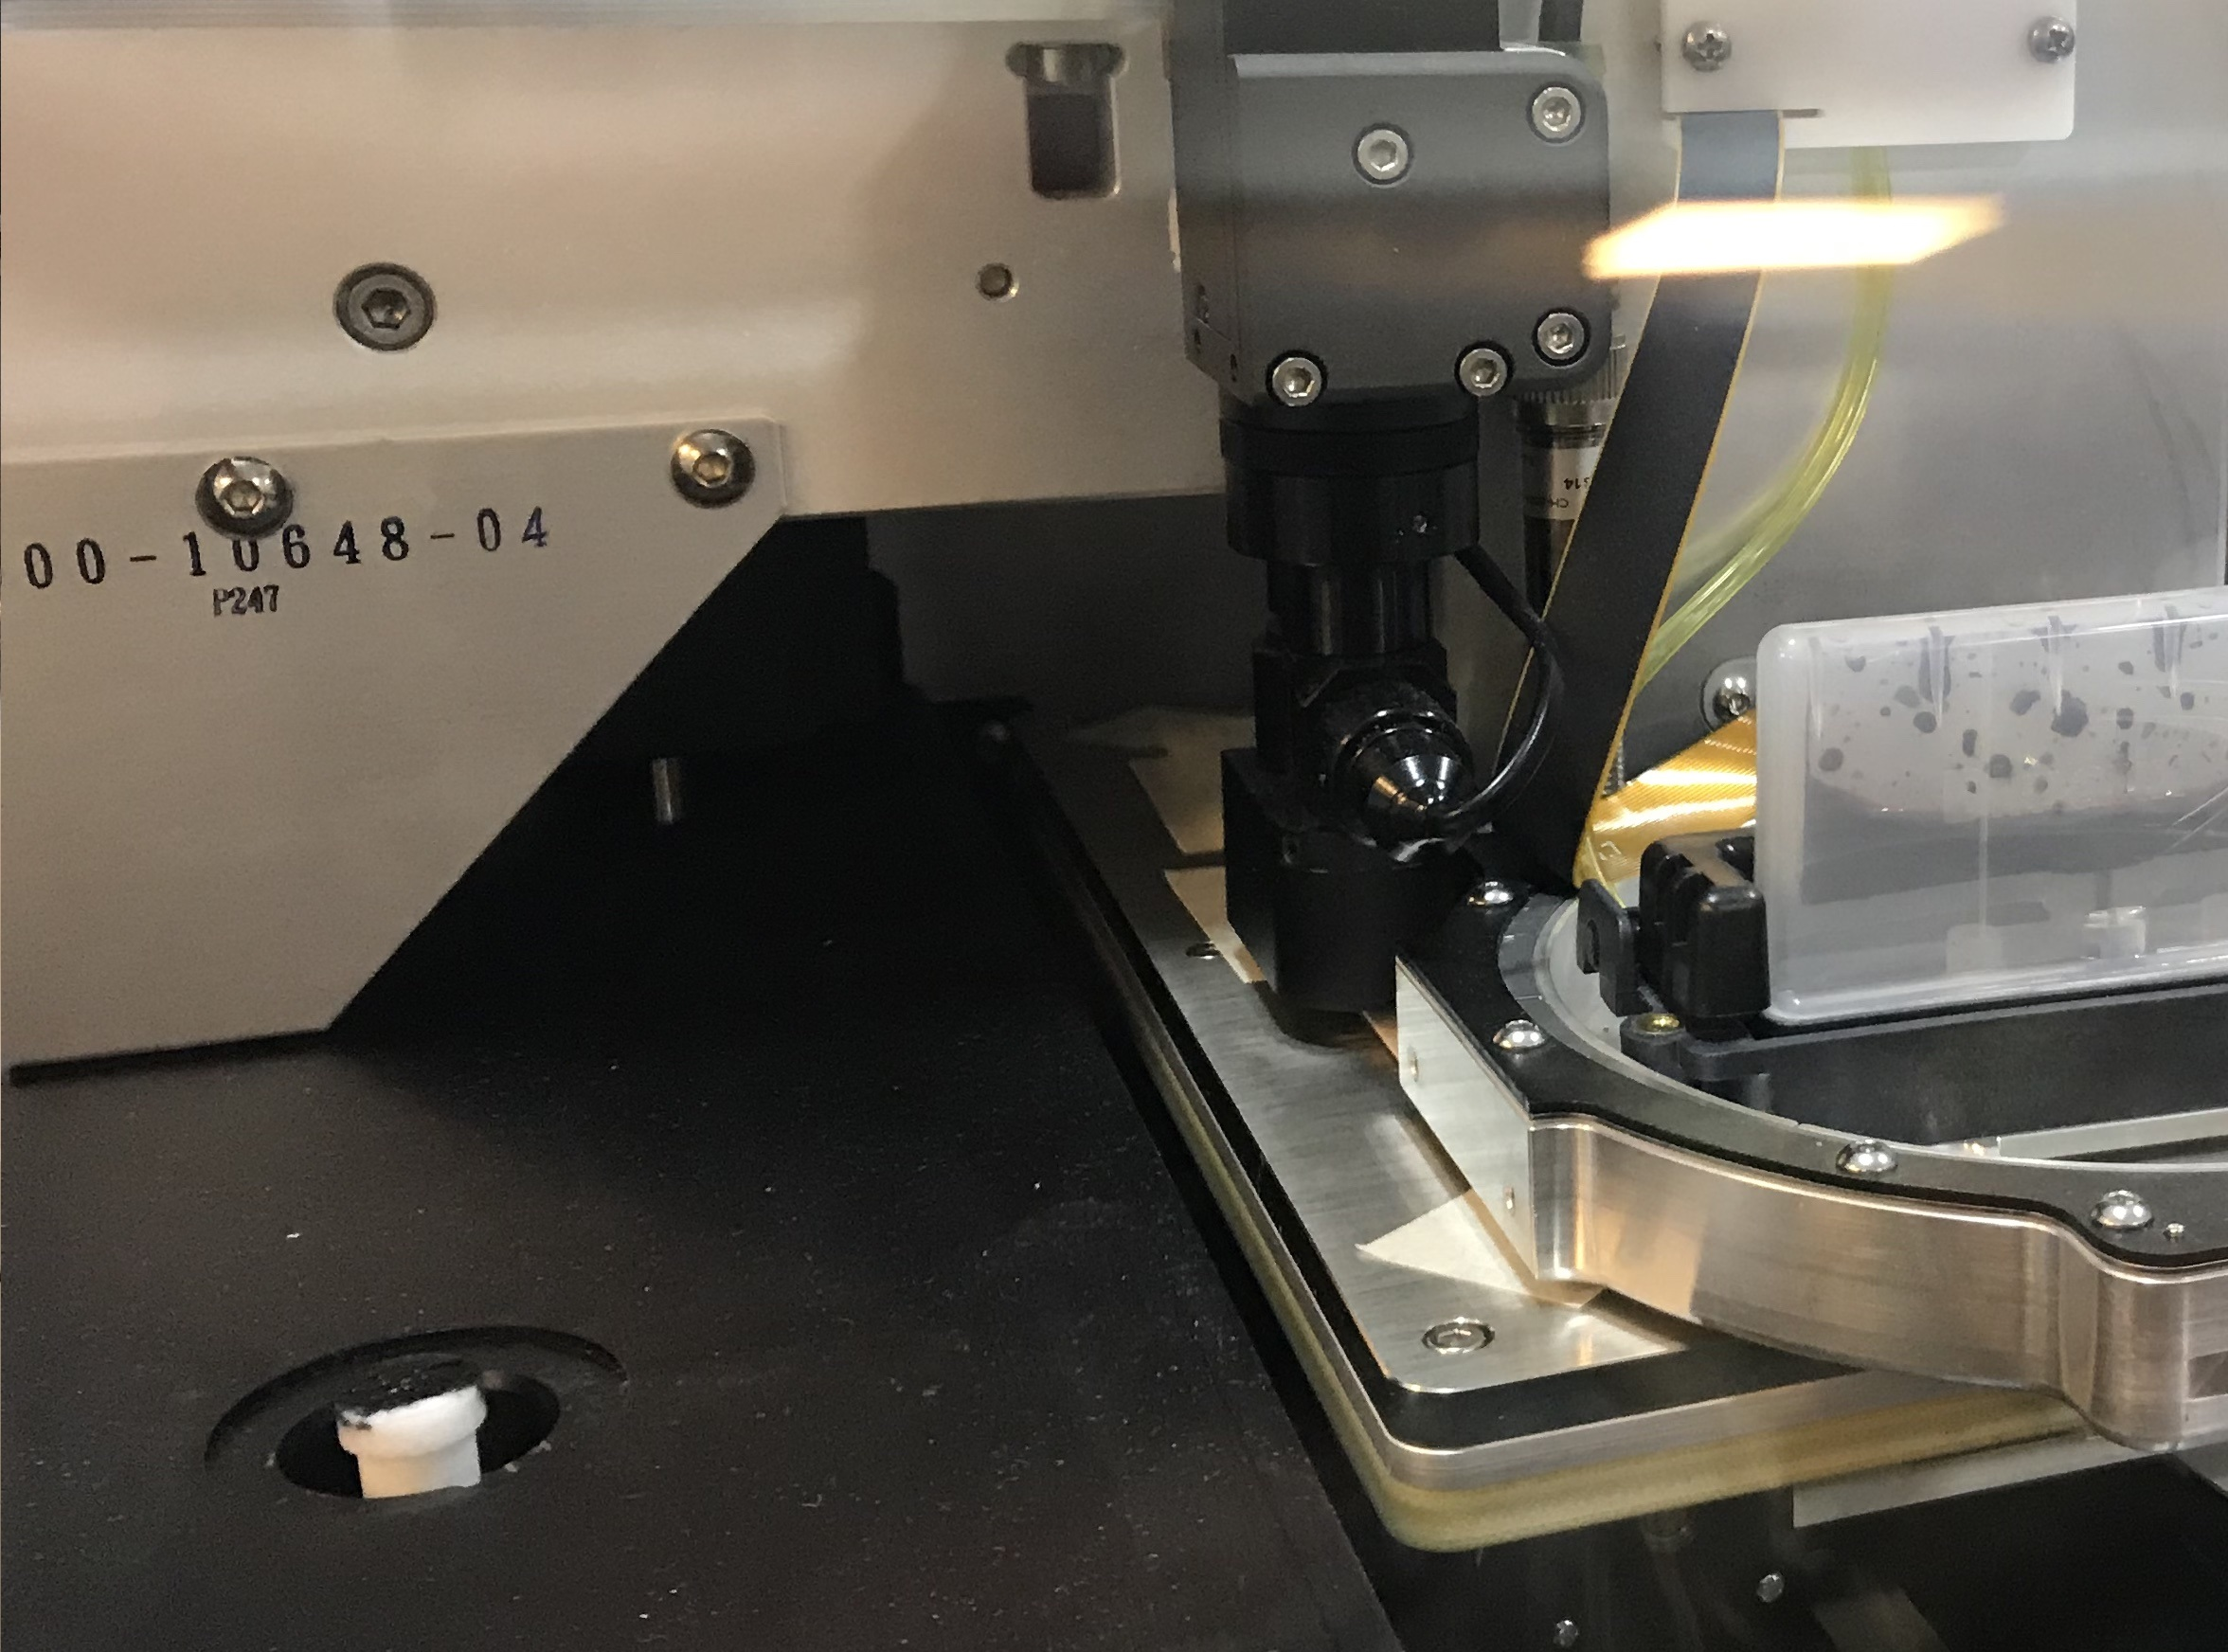
\includegraphics[width=0.5\textwidth]{Figuras/Figura_Orificio_Cleaning_Pad}
  \caption{Ubicación del \textit{Cleaning Pad}.}
  \label{fig:Figura_Orificio_Cleaning_Pad}
\end{figure}

Al cerrar la tapa de la impresora, se finaliza el procedimiento de la instalación del cartucho y el software pide cargar el archivo de configuración, el cual es único para cada tinta. Dentro de este archivo se encuentra la forma de onda que maneja a los eyectores (Figura ~\ref{fig:Figura_Pantalla_Waveform}) y los parámetros ajustados para que sea posible la formación y deposición de las gotas del material. Dentro de estos parámetros se encuentran el límite superior de tensión por cada eyector, la temperatura del cabezal, la presión de vacío para generar el meñisco de tinta, la altura a la que se moverá el cartucho con respecto al sustrato y los ciclos de limpieza antes, durante y después de una impresión (Figura ~\ref{fig:Figura_Configuraciones_cartucho}).

\begin{figure}[H]
  \centering
    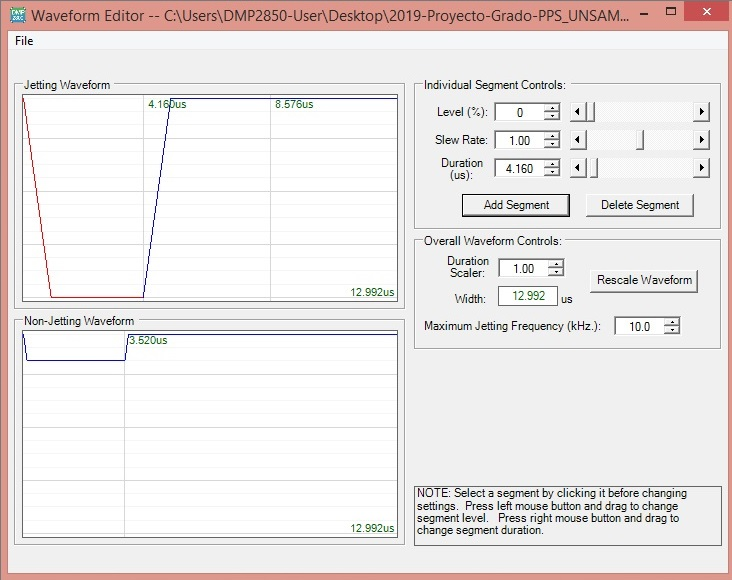
\includegraphics[width=0.5\textwidth]{Figuras/Figura_Pantalla_Waveform}
  \caption{Pantalla de configuración con forma de onda.}
  \label{fig:Figura_Pantalla_Waveform}
\end{figure}

\begin{figure}[H]
  \centering
    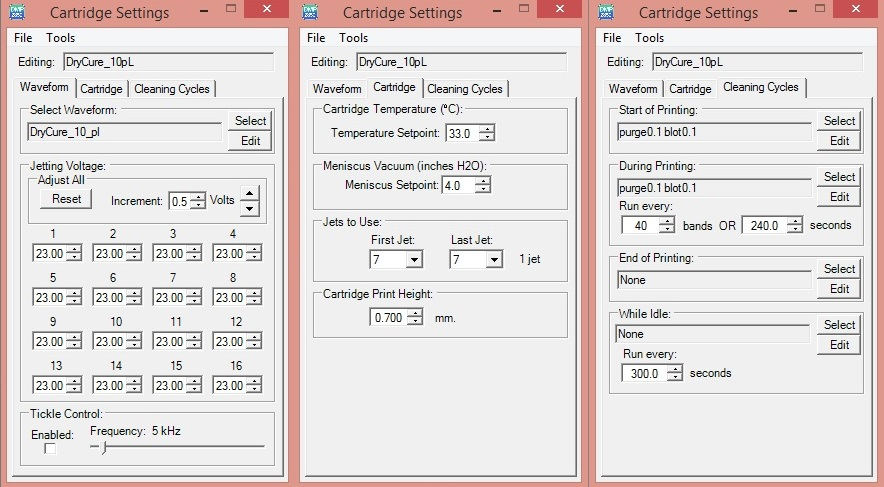
\includegraphics[width=0.8\textwidth]{Figuras/Figura_Configuraciones_cartucho}
  \caption{Pantallas para configuración de parámetros de impresión.}
  \label{fig:Figura_Configuraciones_cartucho}
\end{figure}

Para comprobar el correcto funcionamiento del sistema, se utiliza el \textit{Drop Watcher} donde se puede ver en tiempo real la eyección de las gotas desde los \textit{Nozzles} configurados y a su vez se puede realizar el ajuste de tensiones para equiparar el tiempo de vuelo de los diferentes eyectores (Figura ~\ref{fig:Figura_drop_watcher1}).

\begin{figure}[H]
  \centering
    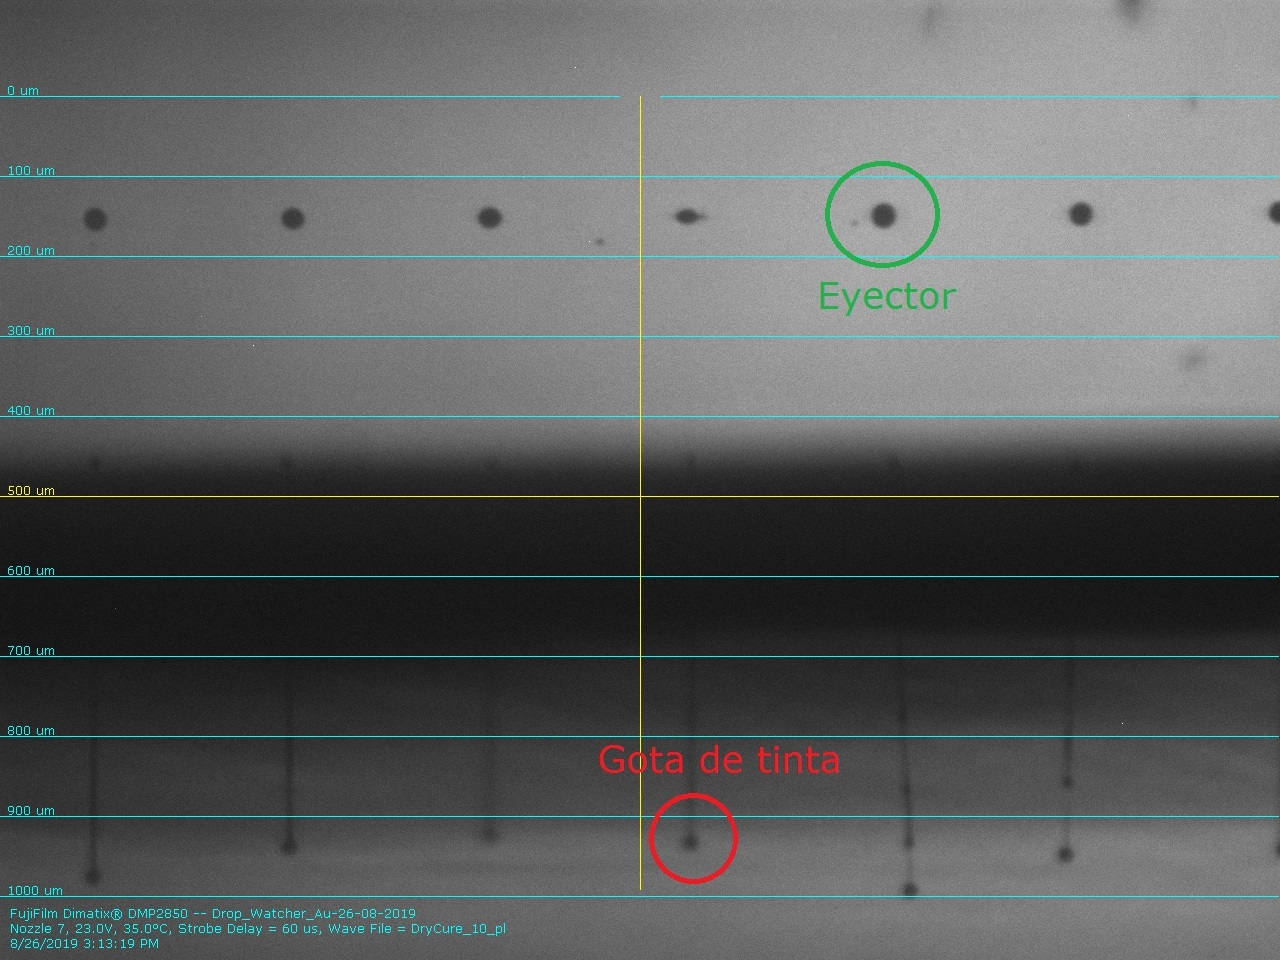
\includegraphics[width=0.5\textwidth]{Figuras/Figura_drop_watcher1}
  \caption{Pantalla de Drop Watcher.}
  \label{fig:Figura_drop_watcher1}
\end{figure}

Una vez finalizado el uso del cartucho, se debe colocar el mismo en forma vertical, de lo contrario el canal que alimenta el cabezal se vaciará de tinta (Figura ~\ref{fig:Figura_canal_cartucho_vacio}). Si esto pasa se deberán realizar varios ciclos de purga o bien rellenar con más tinta, pero no se asegura que el cartucho vuelva a funcionar correctamente.

\begin{figure}[H]
  \centering
    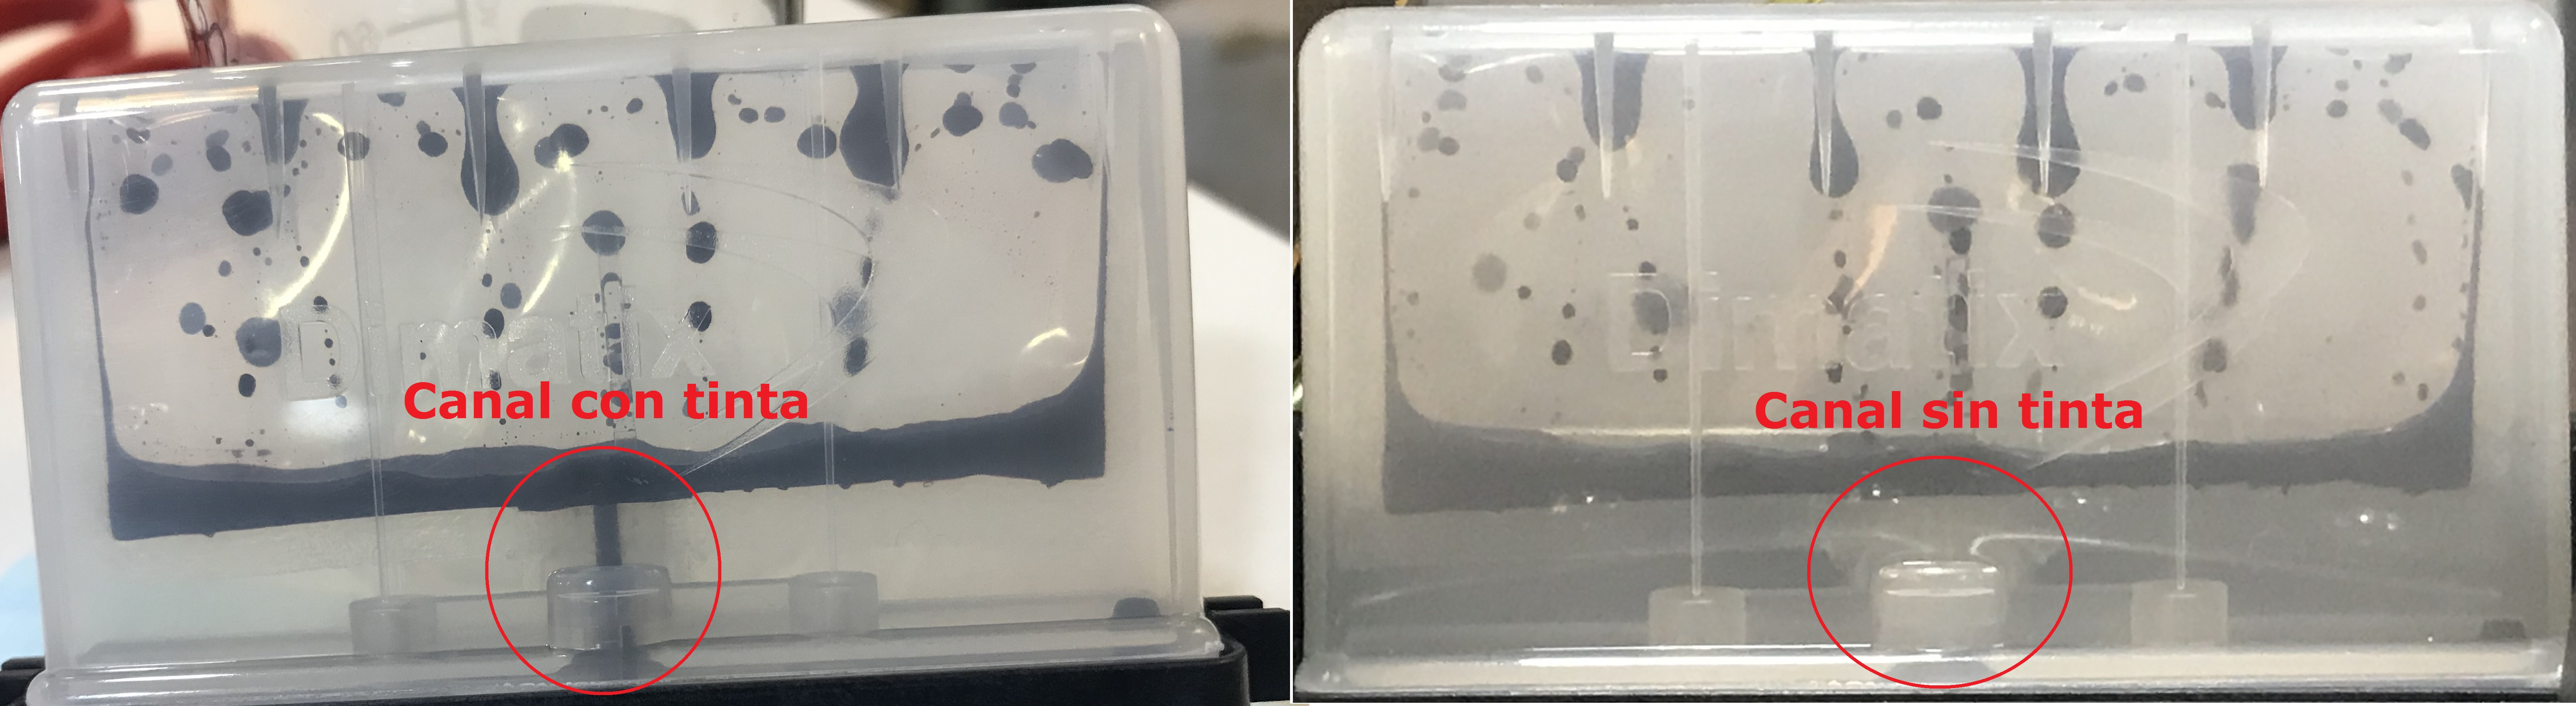
\includegraphics[width=1\textwidth]{Figuras/Figura_canal_cartucho_vacio}
  \caption{Canal de cartucho sin tinta.}
  \label{fig:Figura_canal_cartucho_vacio}
\end{figure}

\section{Sujeción de sustrato y configuración de platina}
La platina de la impresora es una superficie metálica con un arreglo de orificios donde se genera vacío para succionar el sustrato sobre el que se quiere imprimir (Figura ~\ref{fig:Figura_platina}). Si bien el vacío originado en los agujeros es considerable, se debe prestar especial atención en que toda la superficie esté en contacto, de lo contrario la sujeción no será suficiente para mantener dicho sustrato fijo al momento de imprimir. A su vez si todos los orificios no son obstruidos por el sustrato, el sistema no generará la presión negativa estipulada por el fabricante y la fijación no será segura.

\begin{figure}[H]
  \centering
    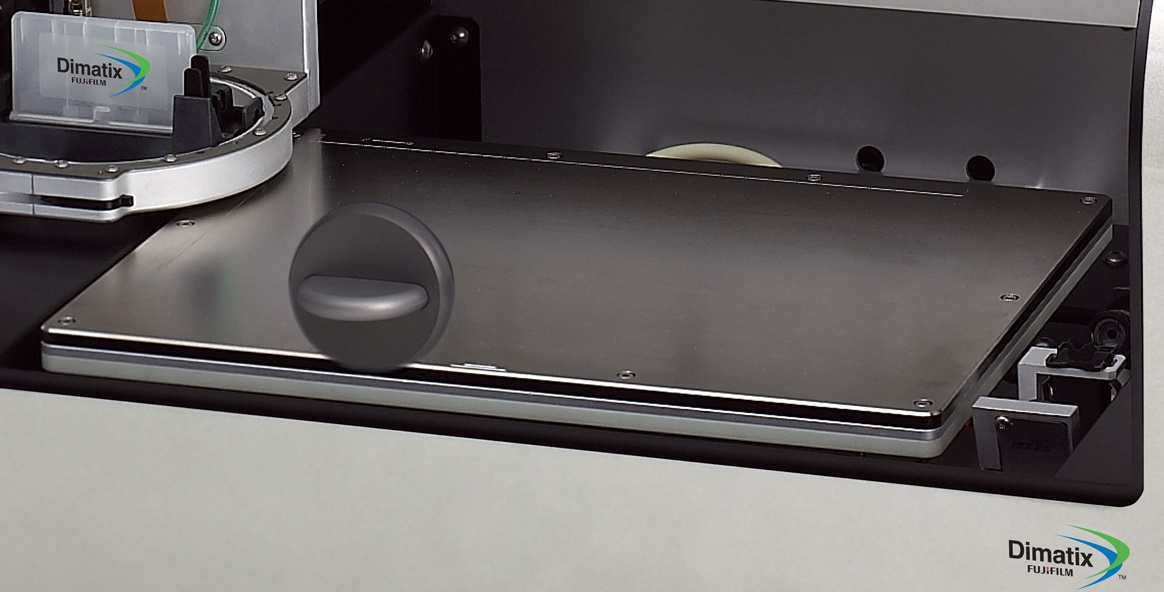
\includegraphics[width=0.5\textwidth]{Figuras/Figura_platina}
  \caption{Platina de impresora Fujifilm Dimatix DMP-2850.}
  \label{fig:Figura_platina}
\end{figure}

Para prevenir estos problemas y asegurar el correcto anclaje de la superficie a imprimir, se utiliza cinta adhesiva de papel.

Es de vital importancia que la base a imprimir no se mueva durante todo el proceso de impresión, prestando la mayor atención luego de realizar la calibración de \textit{Theta}, explicado en el apartado de Puesta a punto y calibración de la impresora, dado que la misma compensa el \textit{offset} angular que pueda generarse entre el sustrato una vez fijado y la platina.

Finalizado el posicionamiento y anclaje del sustrato, se debe configurar el espesor del mismo y la temperatura de la platina mediante el software de la impresora. Si se utilizó cinta adhesiva para la colocación de la muestra, es aconsejable agregar un espesor mayor para evitar el roce del carrete, pérdida de tinta o la rotura del cabezal.